\documentclass[11pt]{article}

\usepackage[margin=1in]{geometry}
\usepackage{amsmath, amssymb}
\usepackage{booktabs}
\usepackage{graphicx}
\usepackage{float}
\usepackage[hidelinks]{hyperref}
\usepackage{natbib}

\graphicspath{{../Figures/}}
\emergencystretch=3em

\title{Bayesian VAR Forecasting and Fiscal Policy Analysis\\ for Switzerland}
\author{Justin Iler and Prathinav Vishnu}
\date{April 2023 \\ \small Revised October 2026}

\begin{document}
\maketitle

\begin{abstract}
\noindent This paper applies a Bayesian vector autoregression (BVAR) with a Minnesota prior to Swiss quarterly data on the short-term interest rate, unemployment and seasonally adjusted, annualized inflation over 2010--2020. The lag length and prior tightness are chosen jointly by maximizing the marginal data density (MDD). In a recursive pseudo-out-of-sample exercise in which every step uses only data available at the forecast origin, the BVAR reduces one-step-ahead mean squared forecast errors relative to a flat-prior (OLS) VAR by a factor of 5 for the interest rate and 1.5 for inflation, and matches it for unemployment. Against a no-change random walk it is about 10 percent more accurate for unemployment and inflation but considerably less accurate for the interest rate, which was pinned near its lower bound for most of the sample. A contractionary monetary policy shock, identified with sign restrictions, raises the interest rate by about 6 basis points, raises unemployment by about 0.11 percentage points and lowers annualized inflation by about 0.14 percentage points on impact, with effects fading within about a year and a half. Iterated forecasts for the 2021 hold-out year track the interest rate closely but miss both the speed of the post-pandemic labor market recovery and the pickup in inflation. Finally, a recursively identified fiscal SVAR on quarterly real government consumption and real GDP (1980--2019) yields a cumulative spending multiplier of about 2.2 on impact and 2.3 after four years, which is large by international standards and should be read as indicative.

\medskip
\noindent\textbf{Keywords:} Bayesian VAR, Minnesota prior, forecasting, impulse responses, monetary policy, fiscal multipliers, Switzerland
\end{abstract}

\newpage

\section{Introduction}

Switzerland's macroeconomy presents a distinctive case study for applied econometric analysis. As a small, open economy with a long tradition of monetary policy independence and exchange rate stability, Switzerland has experienced macroeconomic cycles shaped by both global forces and domestic policy choices. Understanding the transmission of monetary and fiscal shocks to Swiss output, employment and prices is essential for policymakers at the Swiss National Bank (SNB) and the State Secretariat for Economic Affairs (SECO).

This paper develops a Bayesian vector autoregression (VAR) to forecast quarterly Swiss macroeconomic variables and uses structural VARs to study the effects of monetary and fiscal policy shocks. We employ the Minnesota prior for coefficient regularization, with the lag length and prior tightness selected by marginal data density (MDD) maximization, and evaluate forecasts recursively against both a flat-prior VAR and a random walk.

\subsection{Economic Context and Policy Background}

The period 2010--2020 encompasses several significant economic episodes for Switzerland. Following the 2008--09 Great Recession, Swiss monetary policy remained accommodative. In September 2011 the SNB introduced a minimum exchange rate of 1.20 CHF per euro to counter the franc's appreciation. In December 2014 it announced a negative interest rate on sight deposits, and on 15 January 2015 it discontinued the minimum exchange rate and lowered the rate to $-0.75$ percent. Throughout the 2010s, Switzerland experienced low inflation, moderate unemployment (roughly 4.3--5.3 percent) and nominal short-term rates at or below zero.

The COVID-19 pandemic in 2020 triggered a sharp contraction and renewed monetary and fiscal responses. The SNB maintained negative rates and expanded liquidity provision, while the federal and cantonal governments enacted fiscal support programs. By 2021 the economy was recovering, and inflation, which had been subdued for a decade, began to pick up, a pattern that intensified in 2022.

\subsection{Related Literature}

The SNB's own publications \citep{snb2015,snb2020} discuss the motivation for negative rates and unconventional policy. \citet{woodford2003} provides theoretical foundations for monetary policy transmission. \citet{blanchardleigh2013} document substantial heterogeneity in fiscal multipliers across countries and periods.

\citet{litterman1986} introduced the Minnesota prior for VAR forecasting, and \citet{glp2015} provide a modern treatment of prior selection for forecasting. Our forecast evaluation follows their design, comparing a BVAR with a flat-prior VAR and a random walk. Structural identification by sign restrictions follows \citet{canova2002} and \citet{uhlig2005}. Recursive identification of fiscal shocks follows \citet{blanchardperotti2002}. \citet{stockwatson2001} and \citet{delnegro2011} survey VAR methods for macroeconomic analysis.

\subsection{Outline and Contributions}

This paper makes four contributions. First, we show that on a short quarterly sample ($T = 44$), Minnesota-prior shrinkage with MDD-selected lag length and tightness improves on an unrestricted VAR, most clearly for the interest rate, and modestly beats a random walk for unemployment and inflation. It does not beat a random walk for the interest rate, which highlights how little predictable variation that series contains in a negative-rate environment. Second, we identify a contractionary monetary policy shock with theory-consistent sign restrictions and trace its effects on unemployment and inflation. Third, we estimate a Swiss government spending multiplier from quarterly real government consumption over 1980--2019. Fourth, we evaluate the model's iterated forecasts on the 2021 hold-out year.

Section~\ref{sec:data} describes the data and key economic events. Section~\ref{sec:method} outlines the methodology. Section~\ref{sec:results} reports forecast evaluation and impulse responses. Section~\ref{sec:holdout} evaluates the 2021 hold-out forecasts, and Section~\ref{sec:conclusion} concludes.

\section{Time Series Analysis and Economic Events}
\label{sec:data}

\subsection{Data Description}

The main VAR uses three quarterly variables covering 2010 Q1 through 2020 Q4 ($T = 44$ observations):
\begin{itemize}
  \item \textbf{Interest rate (INT):} Swiss 3-month LIBOR, in percent. This variable reflects the monetary policy stance.
  \item \textbf{Unemployment (UR):} Swiss unemployment rate, seasonally adjusted, in percent.
  \item \textbf{Inflation (INFL):} seasonally adjusted, annualized quarter-on-quarter CPI inflation, $400 \times \Delta \log \text{CPI}^{SA}_t$, in percent.
\end{itemize}
We reserve 2021 Q1--Q4 as a hold-out sample.

The raw CPI inflation series is a quarter-on-quarter percent change that is not seasonally adjusted and has a pronounced seasonal pattern: over 2010--2020 average inflation is positive in the first half of the year and negative in the second, and quarter dummies are jointly significant ($p < 0.001$). Following standard practice in the VAR literature, which measures inflation as annualized quarterly log changes of a seasonally adjusted price index \citep{delnegro2011}, we rebuild a CPI index from the raw rates, seasonally adjust it with X-13ARIMA-SEATS over 1990--2021, and take $400 \times \Delta \log$. The adjusted series shows no remaining seasonality ($p = 0.65$). Because the seasonal factors are estimated through 2021, the hold-out year contributes to the adjustment, as it would for officially published seasonally adjusted data.

The fiscal analysis uses two quarterly series from 1980 Q1 to 2019 Q4 ($T = 160$):
\begin{itemize}
  \item \textbf{Government consumption:} real general government final consumption expenditure, seasonally adjusted, in CHF (OECD Main Economic Indicators, via FRED series NAEXKP03CHQ652S).
  \item \textbf{Real GDP:} Swiss real gross domestic product, in millions of CHF.
\end{itemize}
Both enter the fiscal VAR in logs.

\subsection{Key Economic Events and Time Series Features}

\begin{figure}[H]
  \centering
  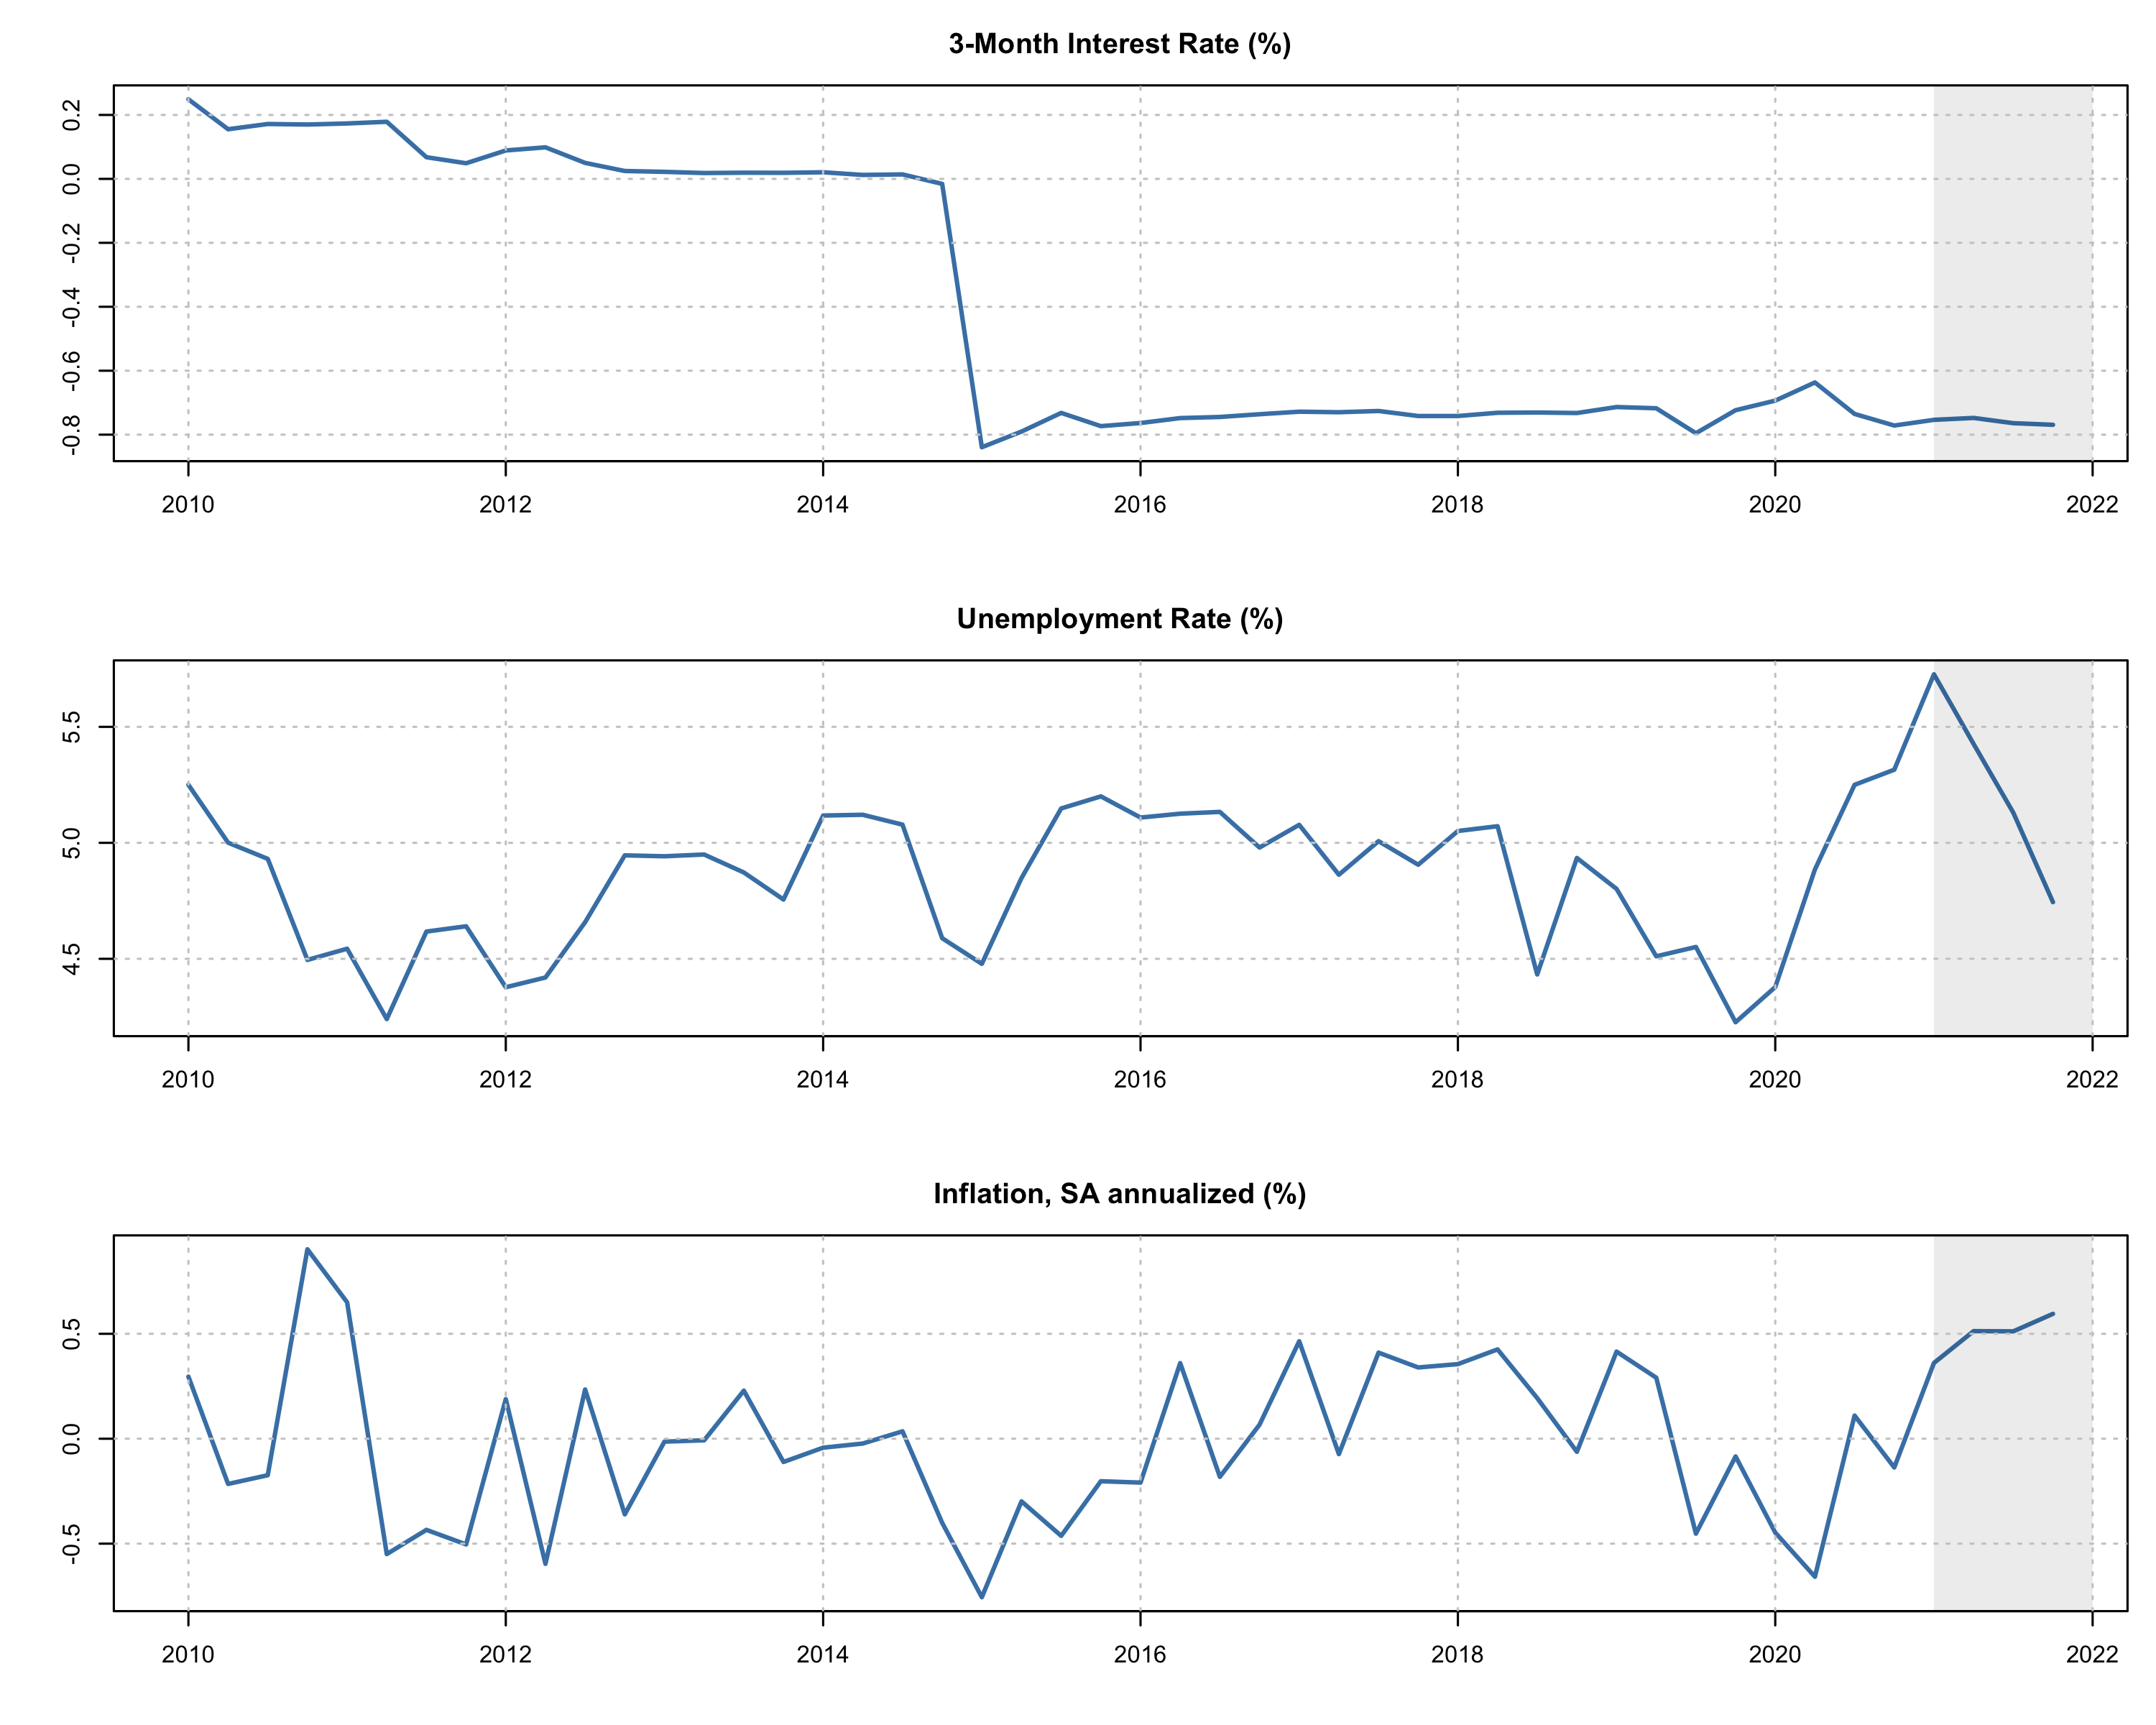
\includegraphics[width=0.9\textwidth]{timeseries.png}
  \caption{Swiss interest rate, unemployment and inflation, 2010 Q1 -- 2021 Q4. The shaded region marks the 2021 hold-out year. Top: the 3-month LIBOR rate drops from slightly above zero to about $-0.75$ percent in early 2015 and stays there through the end of the sample. Middle: unemployment fluctuates between about 4.3 and 5.3 percent, rises during the COVID-19 crisis in 2020 and falls rapidly in 2021. Bottom: seasonally adjusted, annualized inflation fluctuates between about $-0.8$ and $0.9$ percent and rises steadily through 2021.}
  \label{fig:timeseries}
\end{figure}

Several major economic events are reflected in these series:

\paragraph{2010--2011: Post-crisis recovery.} Following the 2008--09 financial crisis, the Swiss economy began recovering in 2010. The SNB kept policy rates near zero. Unemployment declined from about 5.3 percent to about 4.3 percent, and inflation oscillated around zero.

\paragraph{2011--2014: Currency pressure and the exchange rate floor.} From mid-2011 the franc faced strong safe-haven inflows during the European sovereign debt crisis. In September 2011 the SNB introduced the minimum exchange rate of 1.20 CHF per euro, which stabilized the currency for more than three years. Unemployment stayed below about 5 percent and inflation remained very low.

\paragraph{2015: Negative rates and the end of the floor.} On 15 January 2015 the SNB discontinued the minimum exchange rate and lowered its deposit rate to $-0.75$ percent, against the background of global disinflation, falling commodity prices and the ECB's quantitative easing program. The franc appreciated sharply. The 3-month LIBOR rate drops by about 80 basis points in the data, and inflation turns negative.

\paragraph{2016--2019: Persistent negative rates.} The SNB kept its policy rate at $-0.75$ percent throughout this period. Unemployment drifted down, and inflation remained low, in line with persistently low inflation across advanced economies.

\paragraph{2020: COVID-19.} The pandemic induced a sharp contraction in spring 2020. The SNB expanded liquidity provision, and the government enacted substantial fiscal support, including short-time work compensation and business loans. Interest rates remained negative. Unemployment rose above 5 percent by the end of the year and continued to rise into early 2021 before falling quickly.

\subsection{Summary Statistics}

\begin{table}[H]
  \centering
  \caption{Summary statistics (quarterly variables, original scale, 2010--2020)}
  \label{tab:summary}
  \begin{tabular}{lcccc}
    \toprule
    Variable & Mean & Std.\ dev. & Min & Max \\
    \midrule
    INT (\%)  & $-0.37$ & 0.42 & $-0.84$ & 0.25 \\
    UR (\%)   & 4.84    & 0.30 & 4.23    & 5.32 \\
    INFL (\%) & $-0.03$ & 0.37 & $-0.76$ & 0.90 \\
    \bottomrule
  \end{tabular}
\end{table}

The negative mean interest rate reflects the negative-rate regime after 2015. Unemployment is stable relative to its level (coefficient of variation about 6 percent). Annualized inflation averages essentially zero, with quarter-to-quarter fluctuations of a few tenths of a percentage point.

\subsection{Stationarity}

\begin{table}[H]
  \centering
  \caption{Unit-root and stationarity tests. ADF: augmented Dickey--Fuller statistic (null: unit root; lags chosen by BIC, up to 4), with an intercept for the monetary variables and an intercept and trend for the fiscal levels. KPSS: $p$-value of the KPSS test (null: level or trend stationarity).}
  \label{tab:stationarity}
  \begin{tabular}{llcccl}
    \toprule
    Series & Sample & ADF & 5\% c.v. & KPSS $p$ & Conclusion \\
    \midrule
    Interest rate          & 2010--2020 & $-1.39$ & $-2.93$ & 0.01   & nonstationary (level shift) \\
    Unemployment           & 2010--2020 & $-2.83$ & $-2.93$ & $>0.10$ & borderline \\
    Inflation (SA, ann.)   & 2010--2020 & $-3.98$ & $-2.93$ & $>0.10$ & stationary \\
    $\Delta$ Interest rate & 2010--2020 & $-4.67$ & $-1.95$ & $>0.10$ & stationary \\
    $\Delta$ Unemployment  & 2010--2020 & $-5.31$ & $-1.95$ & $>0.10$ & stationary \\
    log gov.\ consumption  & 1980--2019 & $-1.64$ & $-3.43$ & 0.01   & I(1) \\
    log real GDP           & 1980--2019 & $-2.93$ & $-3.43$ & 0.02   & I(1) \\
    $\Delta$ log gov.\ consumption & 1980--2019 & $-5.28$ & $-2.88$ & 0.02 & stationary \\
    $\Delta$ log real GDP  & 1980--2019 & $-7.77$ & $-2.88$ & $>0.10$ & stationary \\
    \bottomrule
  \end{tabular}
\end{table}

Table~\ref{tab:stationarity} reports unit-root tests. Seasonally adjusted inflation is stationary. The interest rate is nonstationary over 2010--2020, which mostly reflects the one-time shift to negative rates in 2015, and unemployment is borderline; both are stationary in first differences. The fiscal variables are integrated of order one, with stationary growth rates.

We nonetheless estimate both VARs in levels, as is common in the Bayesian VAR literature \citep{delnegro2011, glp2015} and in the fiscal SVAR of \citet{blanchardperotti2002}. A levels VAR nests the differenced specification: when the autoregressive coefficients of a variable sum to one, its equation is equivalent to one in first differences. The Minnesota prior is designed for persistent series, centering each variable on a random walk and adding sum-of-coefficients and co-persistence dummy observations, and Bayesian inference remains valid in the presence of unit roots. Estimating in levels also preserves long-run relationships, such as the stable ratio of government consumption to GDP, that differencing would discard.

\section{Methodology}
\label{sec:method}

\subsection{VAR Specification}

The reduced-form VAR for $y_t = (\text{INT}_t, \text{UR}_t, \text{INFL}_t)'$ is
\begin{equation}
  y_t = \Phi_0 + \Phi_1 y_{t-1} + \dots + \Phi_p y_{t-p} + u_t, \qquad u_t \sim N(0, \Sigma).
\end{equation}
Each variable is standardized to zero mean and unit variance using the moments of the estimation sample, and forecasts and impulse responses are converted back to original units. In the recursive forecasting exercise, the moments are recomputed at every forecast origin from data available at that date.

\subsection{Minnesota Prior}

The Minnesota prior centers each equation on a univariate random walk and shrinks cross-variable and higher-lag coefficients toward zero. It is implemented with dummy observations, which yield a conjugate Normal--Inverse-Wishart (MNIW) prior. Its hyperparameters are $\lambda_1$ (overall tightness), $\lambda_2$ (lag decay), $\lambda_3$ (prior on $\Sigma$), $\lambda_4$ (sum-of-coefficients) and $\lambda_5$ (co-persistence). We fix $\lambda_2 = 4$ and $\lambda_3 = \lambda_4 = \lambda_5 = 1$. The scale and level of the dummy observations are computed from a pre-sample consisting of the first five quarters, which are not used in the likelihood.

\subsection{Lag Length and Hyperparameter Selection}

We choose the lag length $p$ and the tightness $\lambda_1$ jointly by maximizing the log marginal data density over
\[
  p \in \{1, 2, 3, 4\}, \qquad \lambda_1 \in \{0.05, 0.1, 0.2, 0.5, 1, 2, 5, 10\}.
\]
All candidate models are evaluated on the same estimation sample, so their MDDs are comparable. The MDD is available in closed form for the MNIW prior (Appendix~\ref{app:mdd}).

\subsection{Posterior Inference and Forecasting}

Given the selected prior, the posterior is again MNIW. We draw $M = 1{,}000$ times from it: $\Sigma$ from an inverse Wishart, then $\Phi$ from a matrix-normal conditional on $\Sigma$.

\paragraph{Recursive evaluation.} For each forecast origin $t$ from 2013 Q1 to 2020 Q3, using only data up to $t$, we (i) standardize the data, (ii) select $p$ and $\lambda_1$ by MDD, (iii) draw from the posterior and (iv) form the one-step-ahead point forecast as the posterior mean. This follows the forecasting procedure of \citet{glp2015}. We compare the BVAR with two benchmarks:
\begin{itemize}
  \item a flat-prior VAR estimated by OLS with the same lag length;
  \item a random walk, $\hat y_{t+1|t} = y_t$.
\end{itemize}
Accuracy is measured by mean squared forecast error (MSE) in original units.

\paragraph{Hold-out forecasts.} For 2021, we use the posterior from the full 2010--2020 sample and simulate trajectories one to four quarters ahead, including shocks, for each posterior draw. Point forecasts are the means of these trajectories, and 90\% predictive bands are their 5th and 95th percentiles.

\subsection{Identification of Monetary Policy Shocks}

We identify a contractionary monetary policy shock by sign restrictions on the impact responses: the interest rate rises, unemployment rises and inflation falls. These are the responses New Keynesian theory predicts for a surprise tightening. For each posterior draw $(\Phi^i, \Sigma^i)$, we draw a vector $q$ uniformly from the unit sphere and compute the impact response $\Sigma^i_{tr} q$, where $\Sigma^i_{tr}$ is the lower Cholesky factor of $\Sigma^i$. We keep the draw if the sign restrictions hold, flipping the sign of $q$ if needed so that the interest rate rises. Every posterior draw yielded an admissible rotation. Responses are reported in percentage points for a one-standard-deviation shock, with 90\% pointwise credible bands.

\subsection{Identification of Fiscal Policy Shocks}

Following \citet{blanchardperotti2002}, the fiscal SVAR is a bivariate VAR in log real government consumption $g_t$ and log real GDP $x_t$:
\begin{equation}
  \begin{pmatrix} g_t \\ x_t \end{pmatrix} = c + \delta\, t + \sum_{j=1}^{4} \Phi_j \begin{pmatrix} g_{t-j} \\ x_{t-j} \end{pmatrix} + \Sigma_{tr}\, \epsilon_t.
\end{equation}
It includes a constant and a linear time trend and is estimated by OLS. Spending is ordered first, so government consumption does not respond to non-fiscal shocks within the quarter. Because both variables are in logs, the impulse responses are percentage deviations. We convert them into CHF using the levels of $g$ and $x$ in the last sample quarter and report the cumulative multiplier
\begin{equation}
  \mathcal{M}_H = \frac{\sum_{h=0}^{H} \Delta X_h}{\sum_{h=0}^{H} \Delta G_h} = \frac{\sum_{h=0}^{H} \hat x_h}{\sum_{h=0}^{H} \hat g_h} \cdot \frac{X_T}{G_T},
\end{equation}
where $\hat x_h$ and $\hat g_h$ are the log responses at horizon $h$, and $X_T$ and $G_T$ are the CHF levels of GDP and government consumption in the last sample quarter. All impulse responses are reported up to $H = 16$ quarters.

\section{Results}
\label{sec:results}

\subsection{Lag Length and Hyperparameter Selection}

\begin{table}[H]
  \centering
  \caption{Log marginal data density by lag length and prior tightness (2010--2020)}
  \label{tab:mdd}
  \begin{tabular}{lcccc}
    \toprule
    $\lambda_1$ & $p=1$ & $p=2$ & $p=3$ & $p=4$ \\
    \midrule
    0.05 & $-145.29$ & $-157.60$ & $-163.11$ & $-164.22$ \\
    0.10 & $-143.40$ & $-150.47$ & $-153.37$ & $-153.64$ \\
    0.20 & $-141.33$ & $-144.98$ & $-146.14$ & $-146.16$ \\
    0.50 & $-138.46$ & $-140.45$ & $-140.61$ & $-140.58$ \\
    1.00 & $\mathbf{-136.63}$ & $-137.75$ & $-137.79$ & $-137.78$ \\
    2.00 & $-137.06$ & $-137.53$ & $-137.54$ & $-137.54$ \\
    5.00 & $-143.35$ & $-143.44$ & $-143.44$ & $-143.44$ \\
    10.00 & $-147.65$ & $-147.67$ & $-147.67$ & $-147.67$ \\
    \bottomrule
  \end{tabular}
\end{table}

Table~\ref{tab:mdd} shows that the MDD is maximized at $p = 1$ and $\lambda_1 = 1$, an interior optimum of the grid. In this dummy-observation parameterization, larger $\lambda_1$ means a tighter prior, so the data favor substantial shrinkage toward random walks. Differences across lag lengths are small once the prior is tight, because higher-order lags are shrunk heavily toward zero. In the recursive exercise the same choice, $p = 1$ and $\lambda_1 = 1$, is selected at every one of the 31 forecast origins.

\subsection{Forecast Evaluation (Recursive, 2013--2020)}

\begin{table}[H]
  \centering
  \caption{One-step-ahead mean squared forecast errors (original units), 31 recursive forecast origins.}
  \label{tab:forecast}
  \begin{tabular}{lccccc}
    \toprule
    Variable & BVAR & OLS VAR & Random walk & OLS / BVAR & RW / BVAR \\
    \midrule
    Interest rate & 0.062 & 0.317 & 0.023 & $5.1\times$ & $0.37\times$ \\
    Unemployment  & 0.060 & 0.059 & 0.067 & $1.0\times$ & $1.12\times$ \\
    Inflation     & 0.118 & 0.177 & 0.131 & $1.5\times$ & $1.10\times$ \\
    \bottomrule
  \end{tabular}
\end{table}

Table~\ref{tab:forecast} compares the BVAR with the two benchmarks. Because the MDD selects a single lag, the flat-prior VAR has only four coefficients per equation, and it is a reasonable competitor for unemployment, where the two models are equally accurate. Its main weakness is the interest rate: around the January 2015 rate cut its forecasts swing far from the data (Figure~\ref{fig:forecasts}), and its MSE is five times that of the BVAR. For inflation, shrinkage reduces the MSE by a third.

Against the random walk, the BVAR is about 10 percent more accurate for unemployment and for inflation, but its interest rate MSE is almost three times as large. The interest rate was essentially constant at about $-0.75$ percent from 2015 onward, the ideal case for a no-change forecast, and the BVAR's largest error is the 2015 Q1 rate cut, after which it partly extrapolates the drop. These results echo \citet{glp2015}: shrinkage is what makes VAR forecasting reliable, but for a small system the gains over a random walk are modest.

\begin{figure}[H]
  \centering
  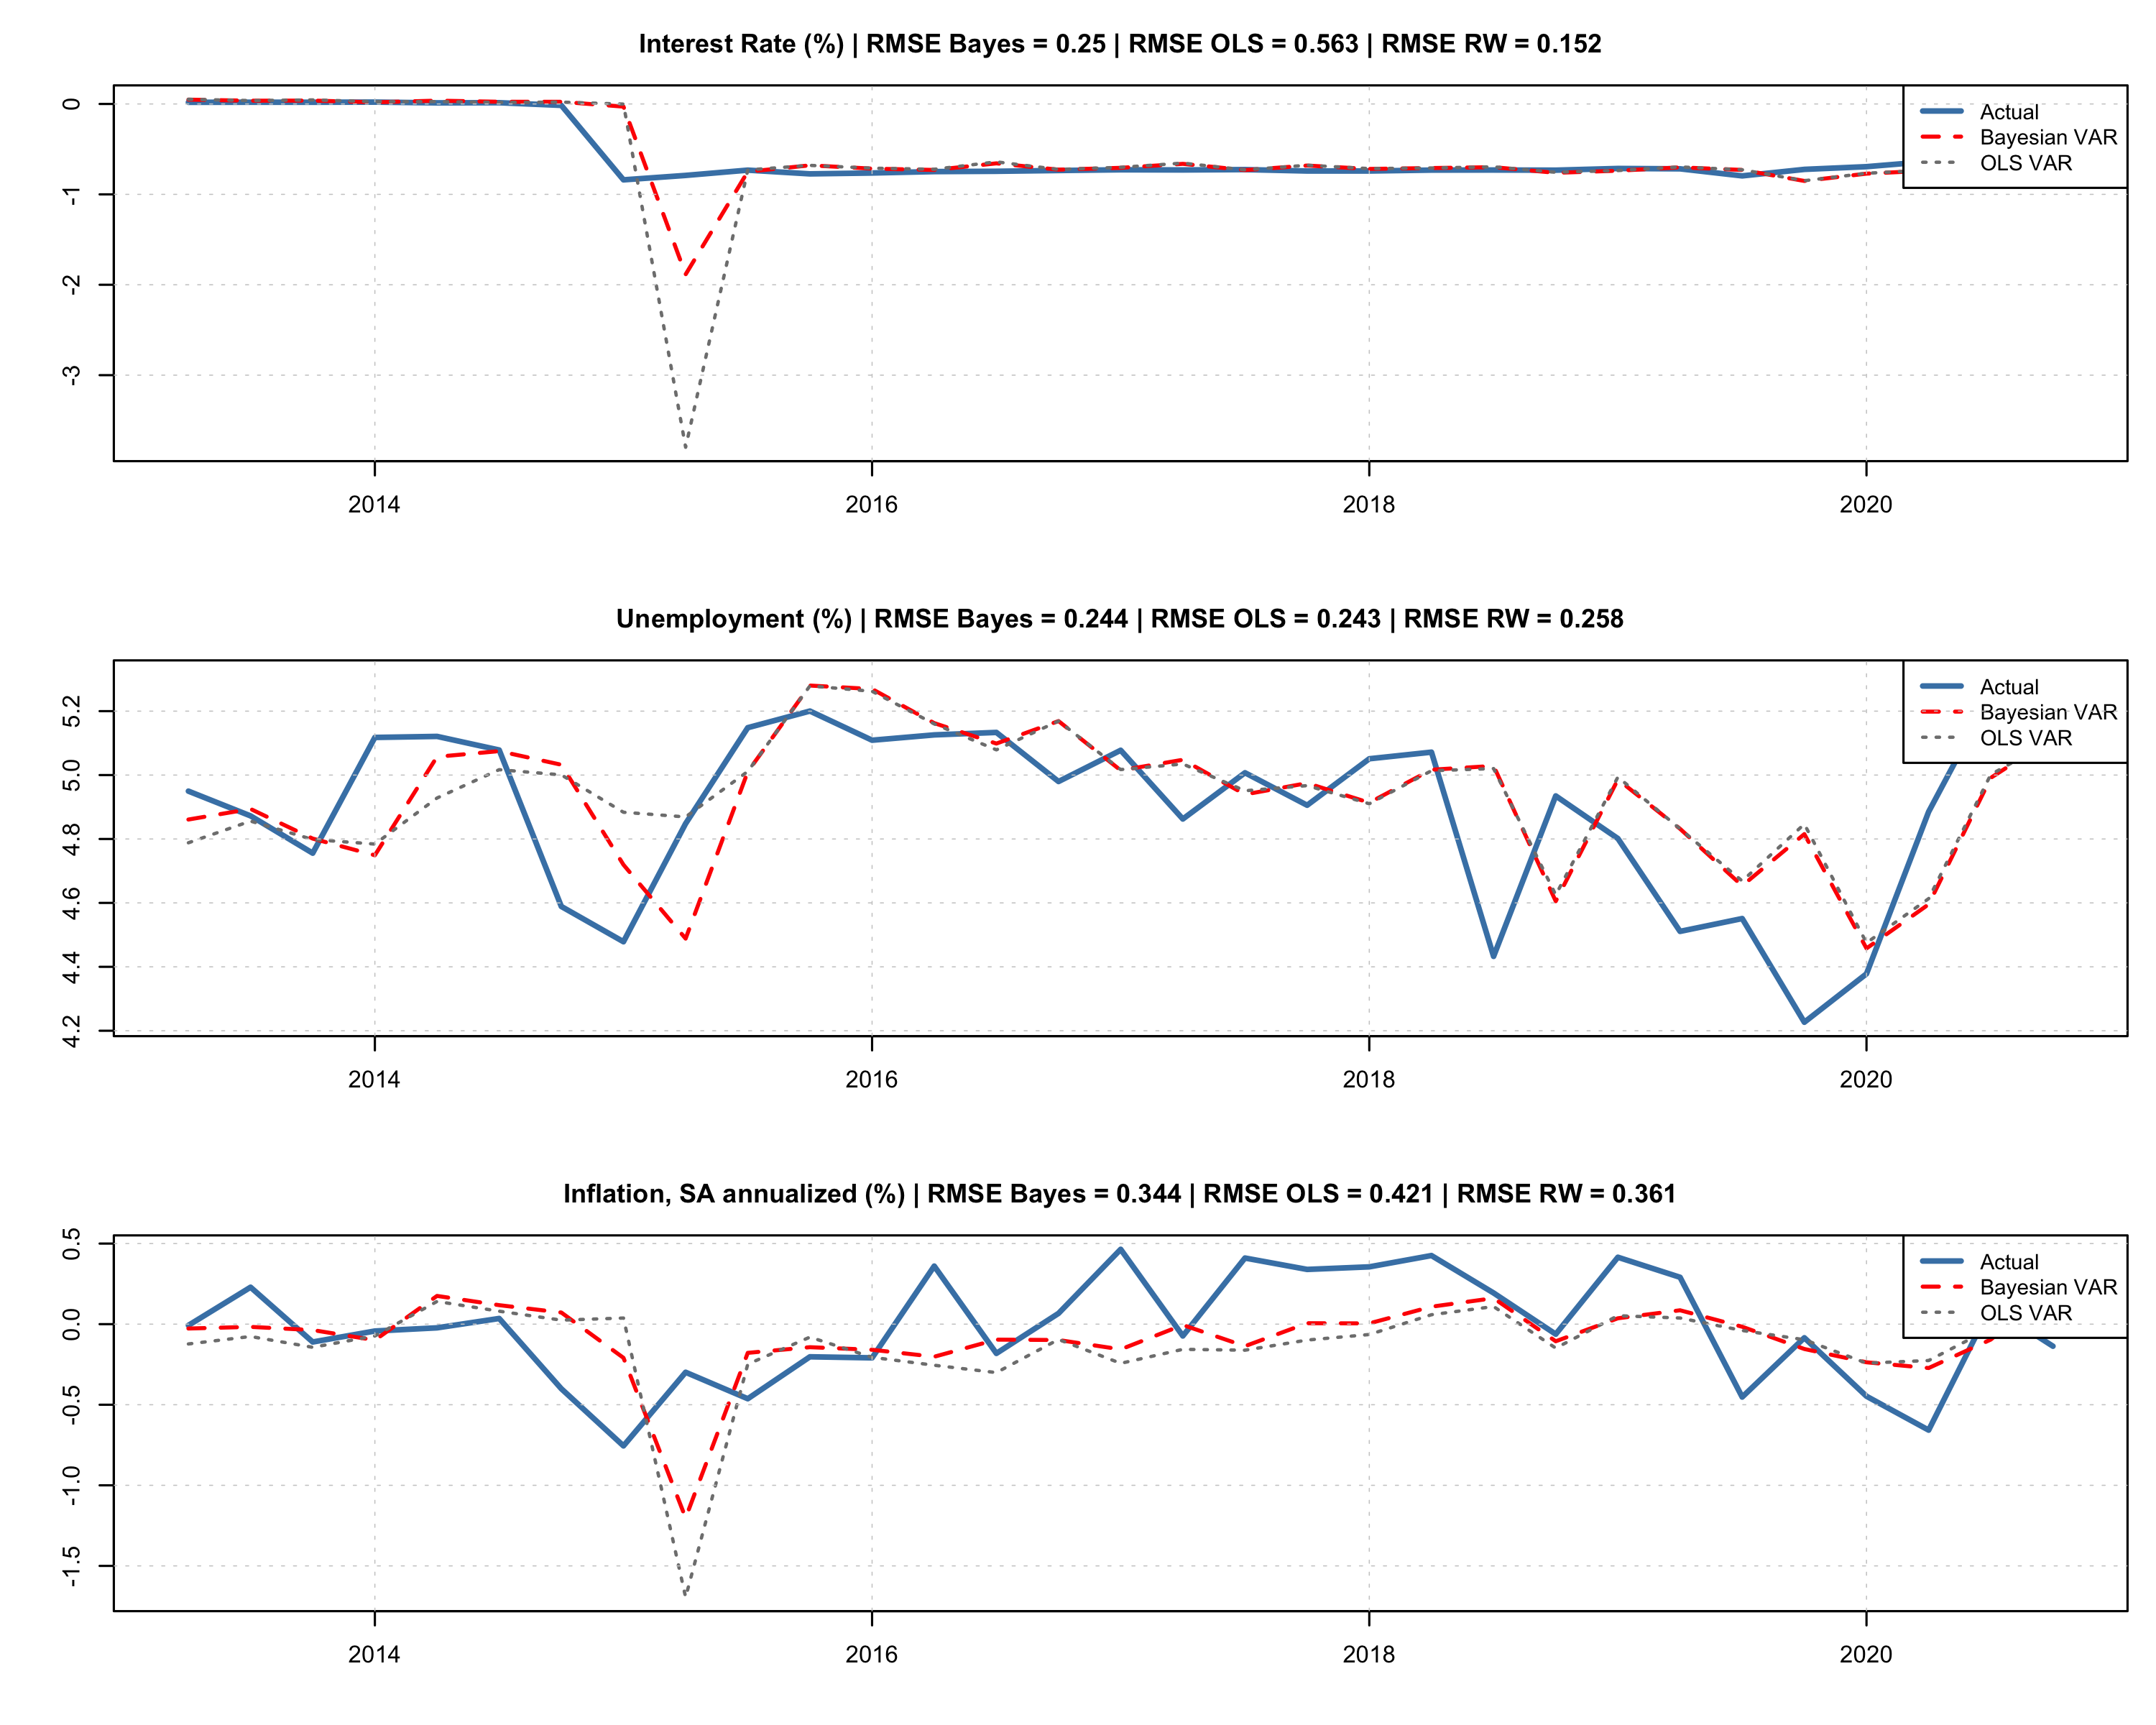
\includegraphics[width=0.9\textwidth]{forecasts.png}
  \caption{Recursive one-step-ahead forecasts, 2013 Q2 -- 2020 Q4 (original units). Blue: actual values. Red dashed: BVAR. Gray dotted: OLS VAR. Panel titles report root mean squared errors for the BVAR, the OLS VAR and the random walk over the comparison sample.}
  \label{fig:forecasts}
\end{figure}

\subsection{Monetary Policy Impulse Responses}

\begin{figure}[H]
  \centering
  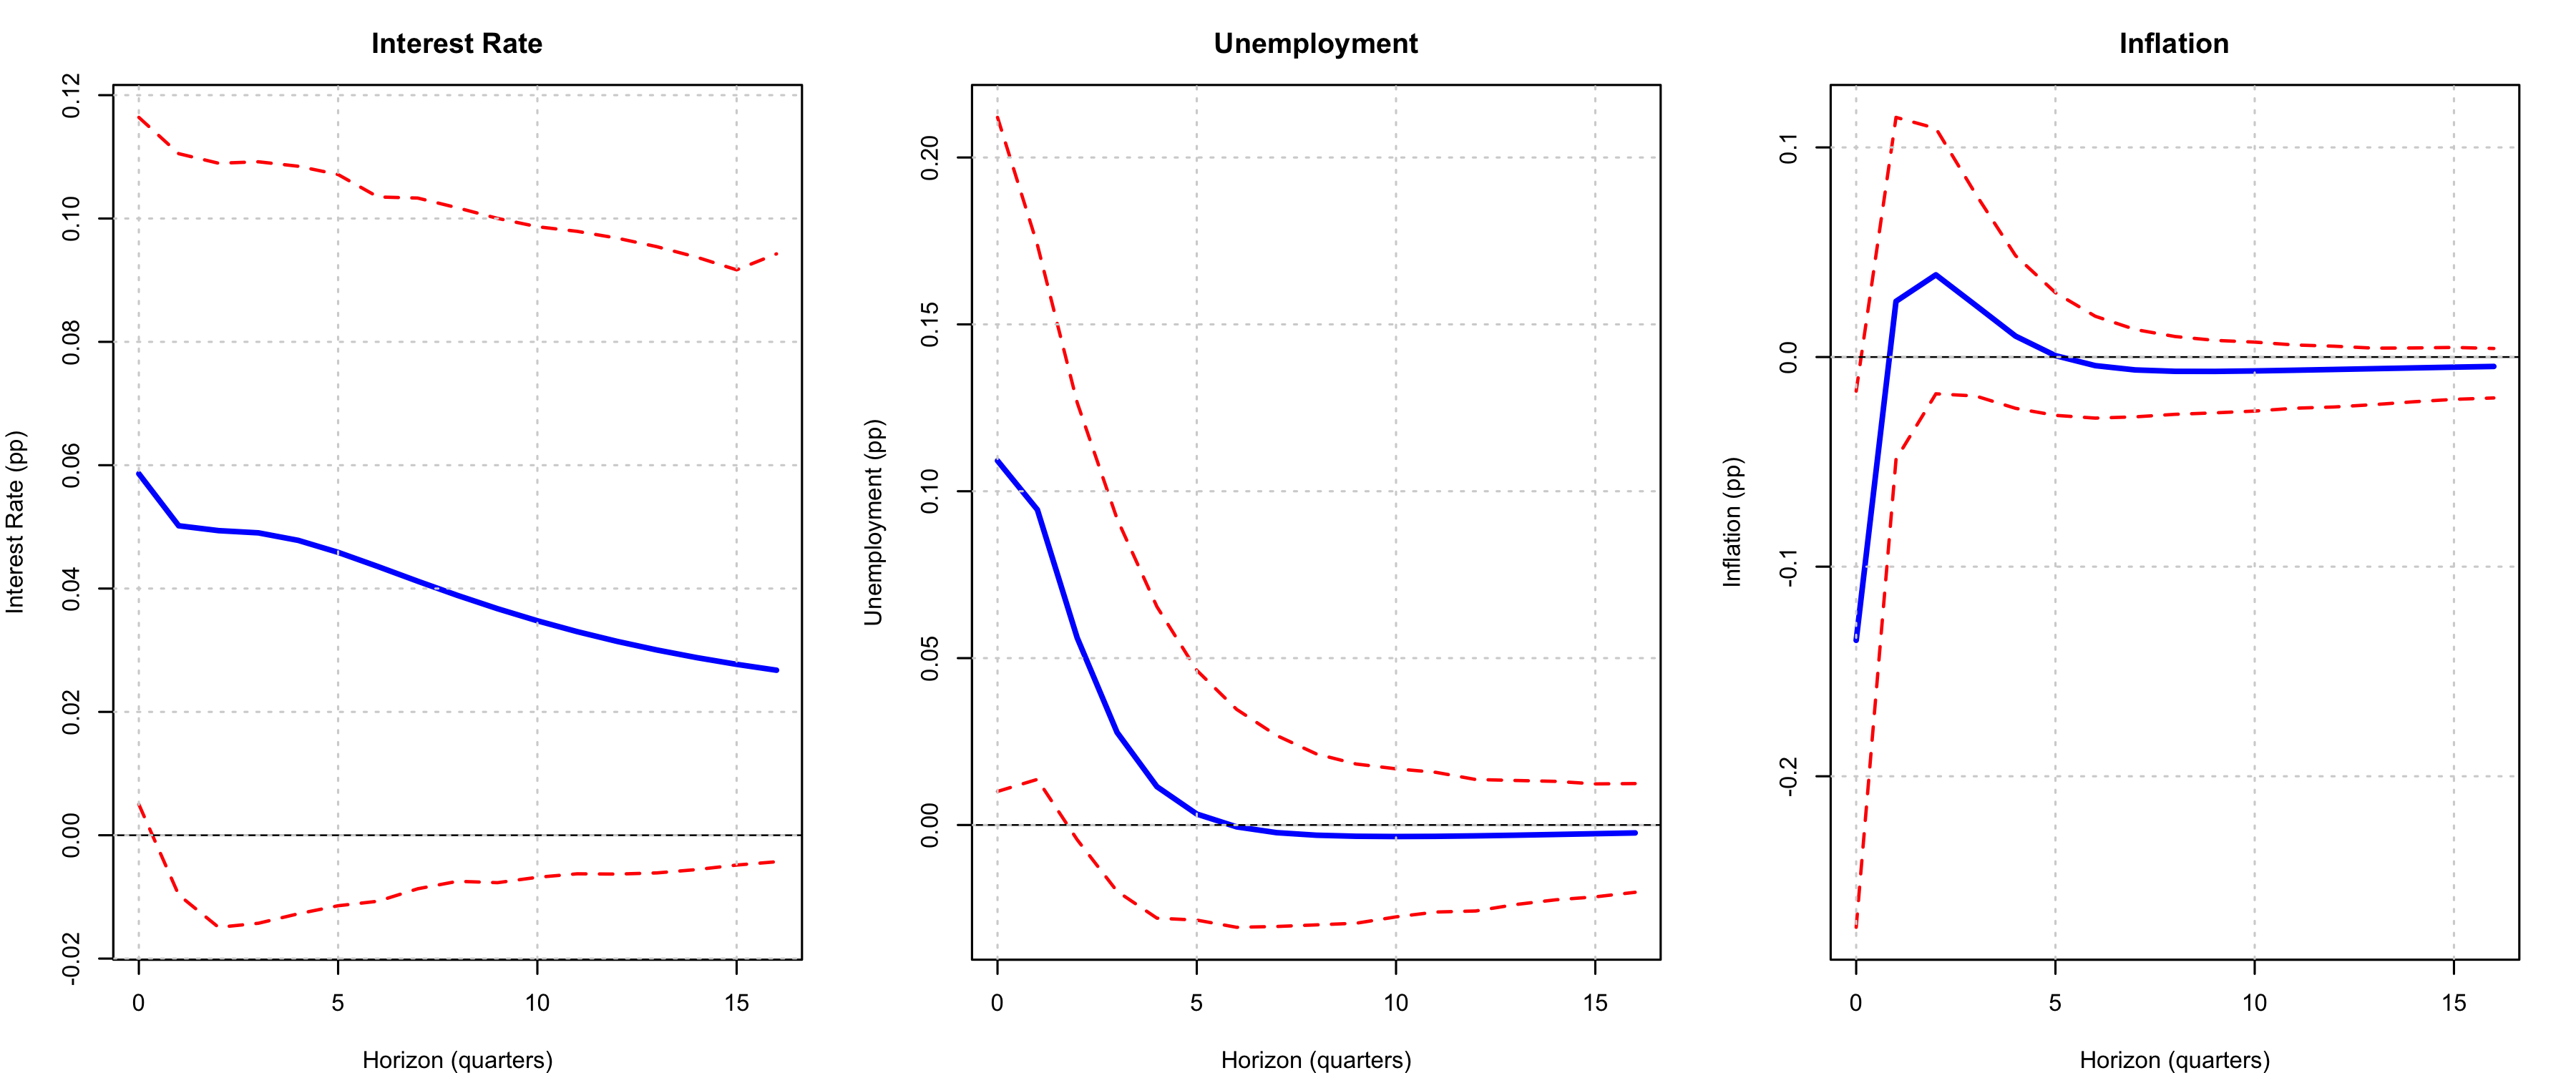
\includegraphics[width=\textwidth]{monetary_irf.png}
  \caption{Responses to a one-standard-deviation contractionary monetary policy shock, identified by sign restrictions on impact (interest rate up, unemployment up, inflation down). Blue: posterior mean. Red dashed: 90\% pointwise credible bands. Units are percentage points (inflation at an annualized rate); the horizon is in quarters.}
  \label{fig:monetary}
\end{figure}

Figure~\ref{fig:monetary} shows the responses to a contractionary monetary policy shock. On impact the interest rate rises by about 6 basis points (90\% band: 0.5 to 12 bp), unemployment rises by 0.11 percentage points (0.01 to 0.21) and annualized inflation falls by 0.14 percentage points ($-0.27$ to $-0.02$). The rate response is persistent, still about 3 bp after four years. Unemployment returns to zero after roughly six quarters. Inflation rebounds slightly above zero in the following quarters, by at most 0.04 percentage points with a band that includes zero, and the response dies out after about five quarters.

The impact signs hold by construction, so the informative content lies in the magnitudes and the dynamics. The shock is small. With the policy rate at its effective lower bound for most of the sample, the data contain little variation in surprise rate changes, and the interest rate band includes values close to zero. As a result, the posterior bands are wide for every variable after the first few quarters. Sign restrictions rule out the price puzzle, an inflation increase after a tightening, on impact by assumption; recursive identification often produces this puzzle \citep{stockwatson2001}. The small, insignificant rebound in later quarters suggests the data contain little information about the inflation response beyond the restriction itself.

\subsection{Fiscal Policy Analysis}

\begin{figure}[H]
  \centering
  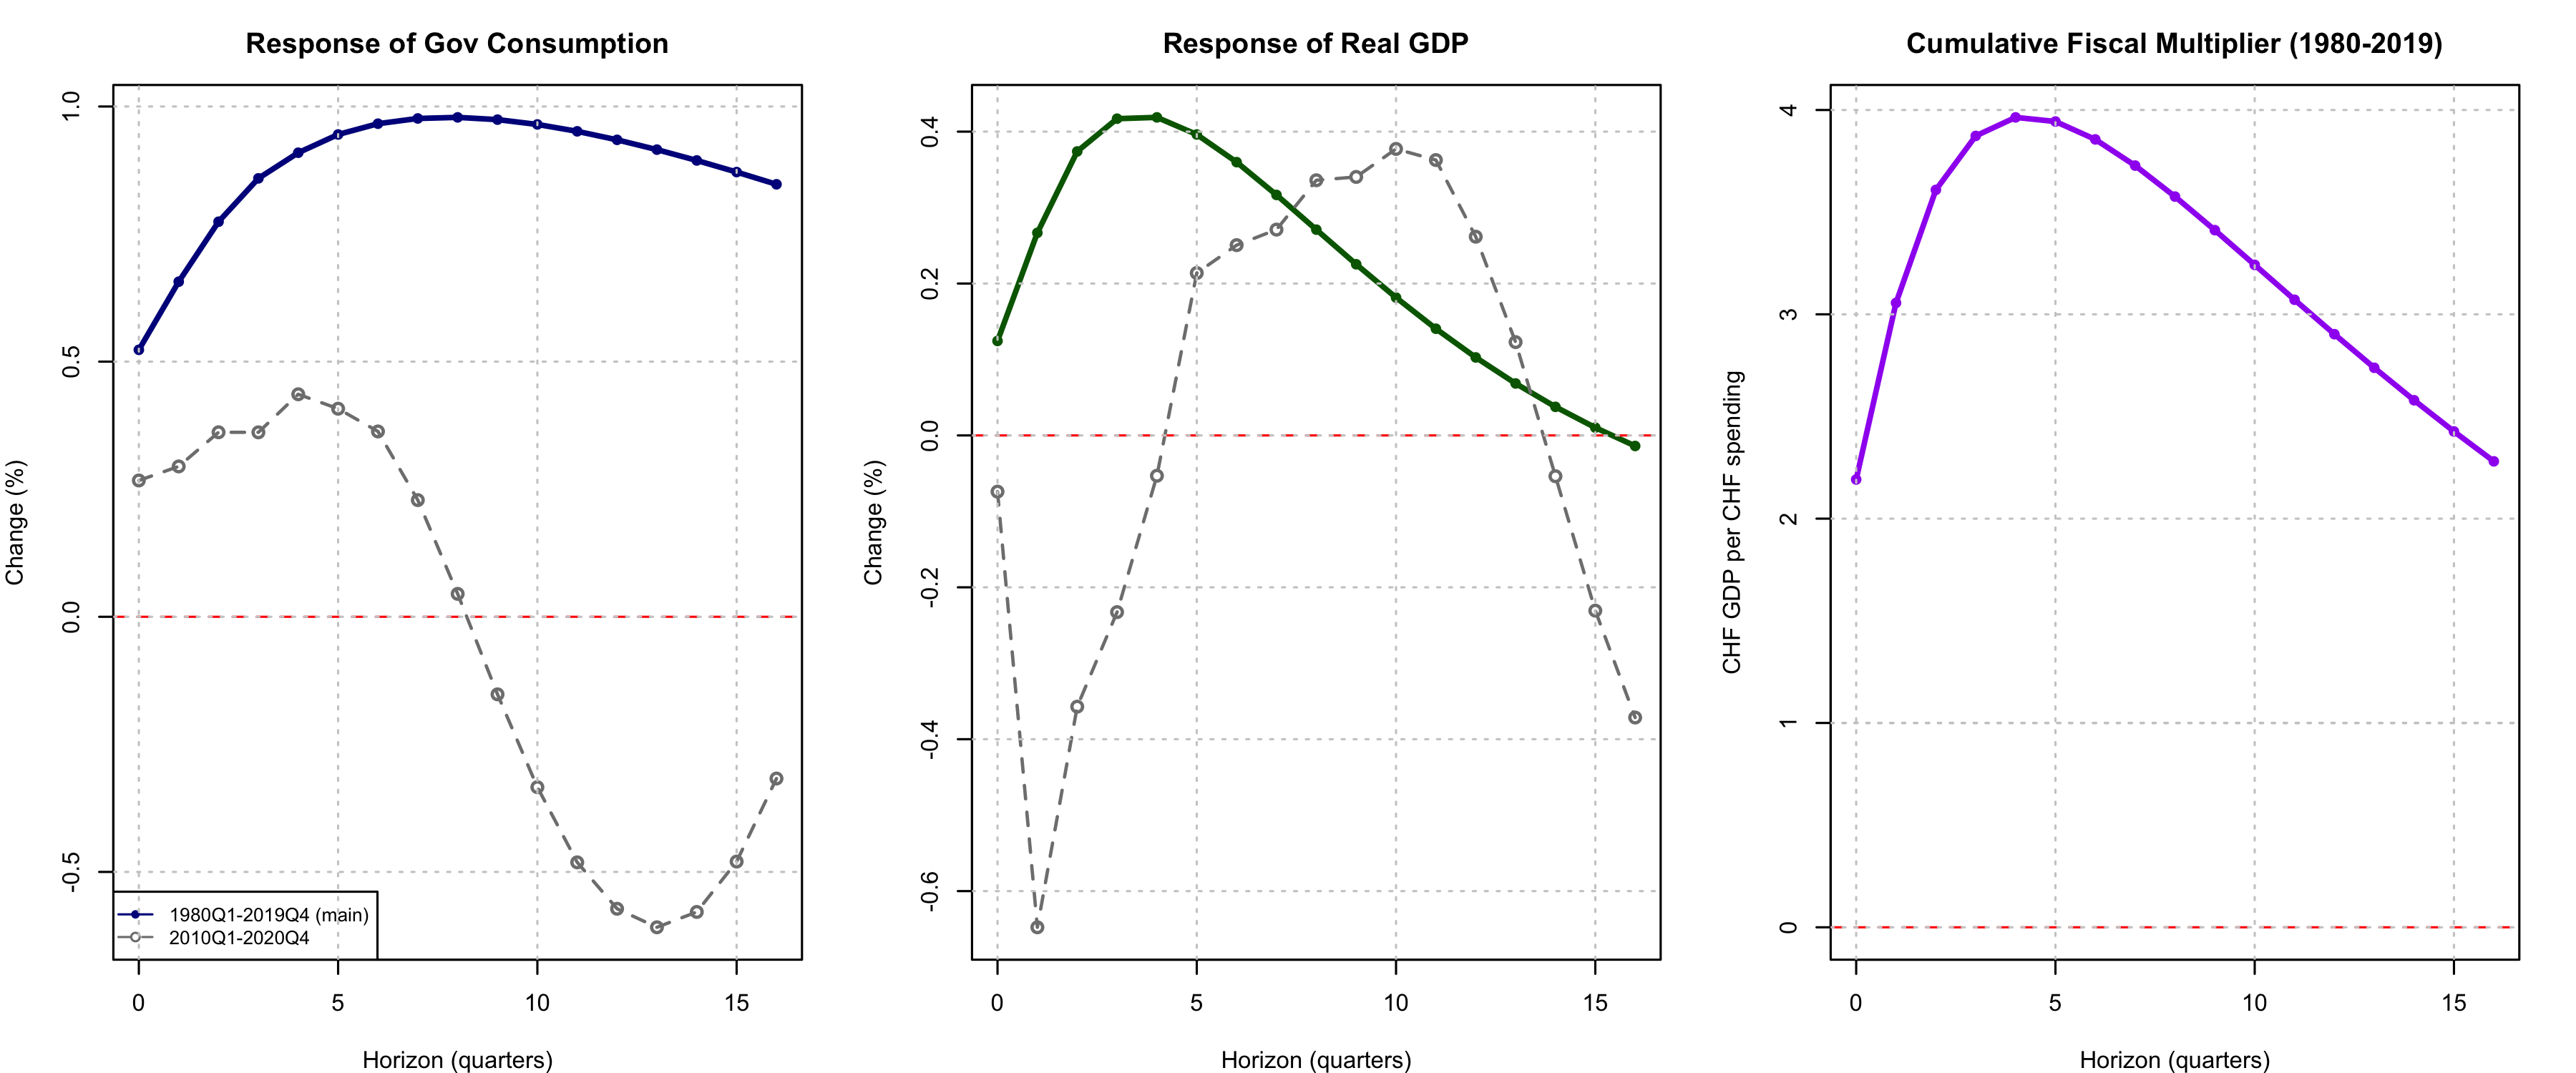
\includegraphics[width=\textwidth]{fiscal_irf.png}
  \caption{Responses to a one-standard-deviation government spending shock in the recursively identified fiscal SVAR (spending ordered first, constant and linear trend, 4 lags). Solid: 1980 Q1 -- 2019 Q4 (main estimate). Gray dashed: the same specification on 2010 Q1 -- 2020 Q4. Right: cumulative multiplier in CHF of GDP per CHF of government consumption for the main estimate.}
  \label{fig:fiscal}
\end{figure}

Figure~\ref{fig:fiscal} reports the fiscal SVAR. In the 1980--2019 sample, a one-standard-deviation spending shock raises real government consumption by 0.52 percent on impact. The response builds to a peak of about 1 percent after two years and decays slowly. Real GDP rises by 0.12 percent on impact, peaks at about 0.42 percent after one year and returns to zero after four years.

Converted into CHF, the cumulative multiplier is about 2.2 on impact, peaks near 4.0 after one year and declines to about 2.3 after four years. These values exceed the multiplier of roughly one typically found for the United States \citep{blanchardperotti2002}. Two features of the Swiss data contribute. First, government consumption is only about 11 percent of GDP, so the elasticity of GDP to spending (about 0.24 on impact) is multiplied by a GDP-to-spending ratio of about 9. Second, recursive identification attributes all contemporaneous comovement between spending and GDP to the spending shock, so any within-quarter response of spending to economic conditions biases the multiplier upward. The estimates come without error bands and should be read as indicative.

On the shorter 2010--2020 window (gray lines), the spending response peaks at about 0.4 percent and turns negative after two years, while GDP initially falls. With only 44 quarterly observations and ten coefficients per equation, the cumulative spending response passes through zero within the four-year horizon, so the CHF multiplier ratio is not meaningful on that sample.

\section{Out-of-Sample Forecasts: 2021 Hold-Out Evaluation}
\label{sec:holdout}

\begin{figure}[H]
  \centering
  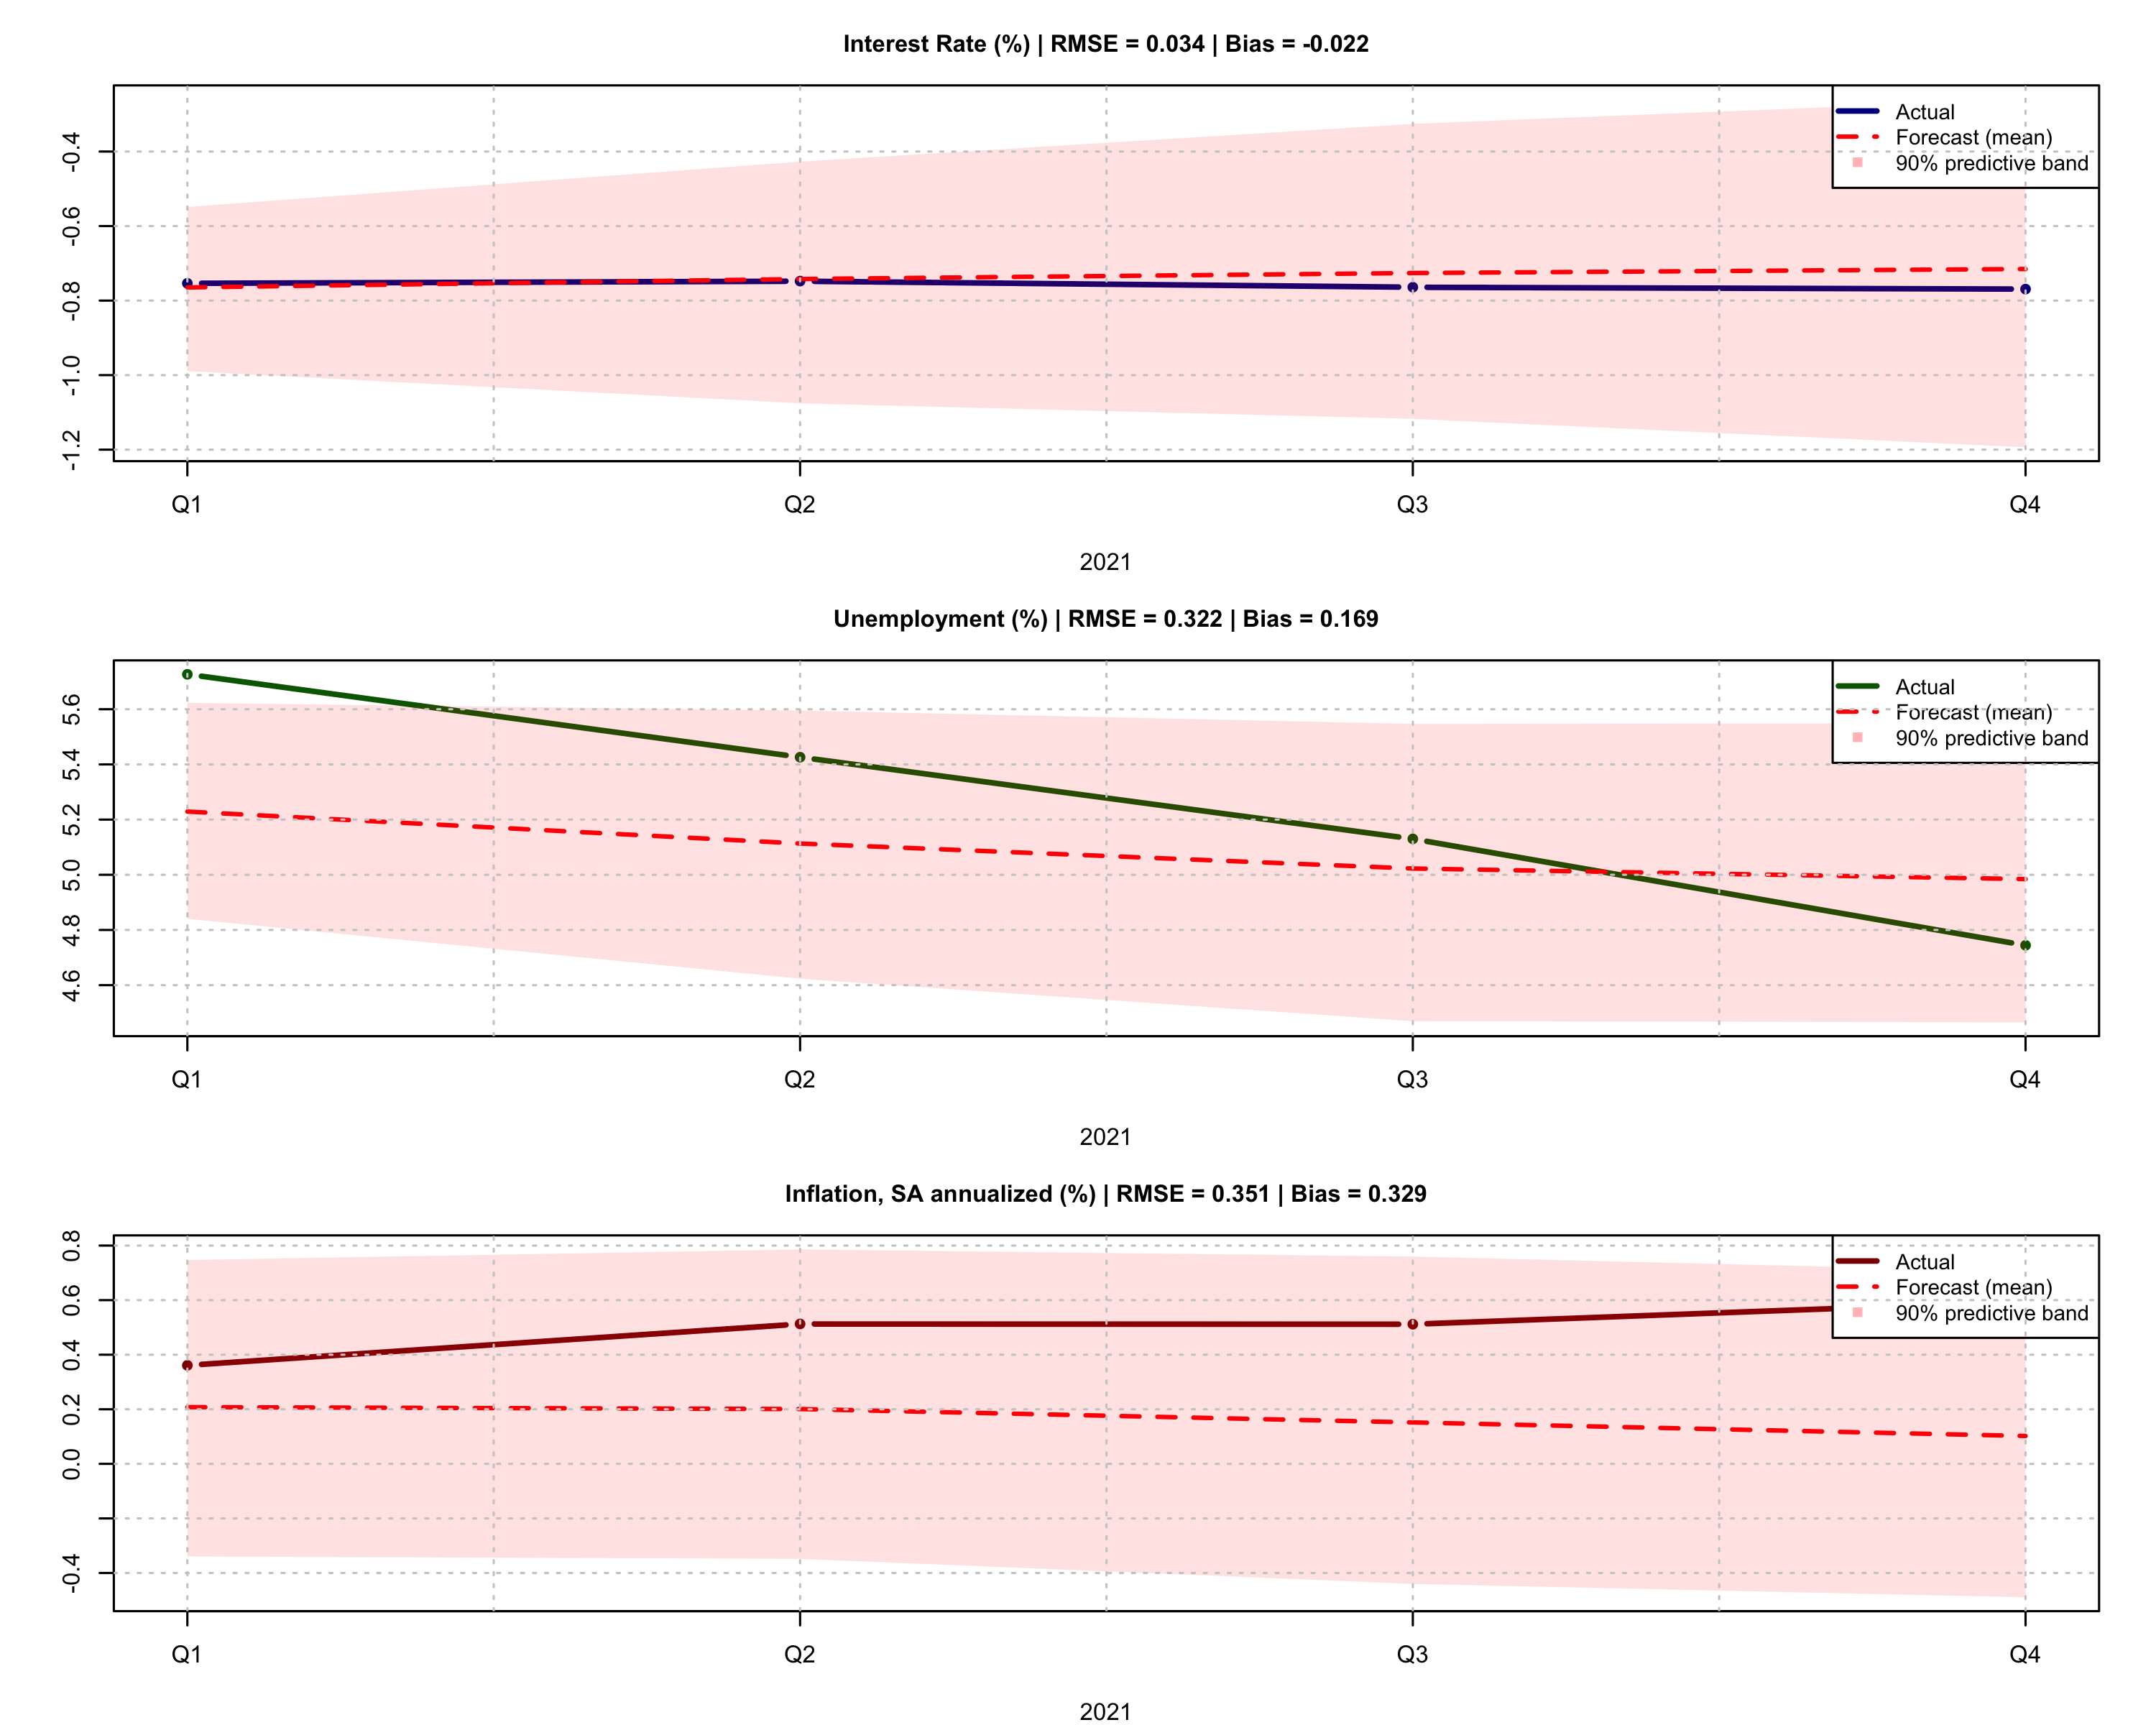
\includegraphics[width=0.9\textwidth]{forecasts_2021.png}
  \caption{Iterated forecasts for 2021 Q1--Q4 from the 2010--2020 posterior. Solid: actual values. Red dashed: posterior predictive mean. Shaded: 90\% predictive band. Panel titles report root mean squared error and bias (actual minus forecast).}
  \label{fig:holdout}
\end{figure}

\begin{table}[H]
  \centering
  \caption{2021 hold-out forecasts (iterated from 2020 Q4) and outcomes}
  \label{tab:holdout}
  \begin{tabular}{lcccccc}
    \toprule
     & \multicolumn{2}{c}{Interest rate} & \multicolumn{2}{c}{Unemployment} & \multicolumn{2}{c}{Inflation} \\
    Quarter & Forecast & Actual & Forecast & Actual & Forecast & Actual \\
    \midrule
    2021 Q1 & $-0.765$ & $-0.754$ & 5.229 & 5.727 & 0.208 & 0.361 \\
    2021 Q2 & $-0.742$ & $-0.748$ & 5.113 & 5.426 & 0.201 & 0.513 \\
    2021 Q3 & $-0.726$ & $-0.764$ & 5.023 & 5.130 & 0.152 & 0.512 \\
    2021 Q4 & $-0.715$ & $-0.769$ & 4.984 & 4.744 & 0.102 & 0.595 \\
    \midrule
    RMSE & \multicolumn{2}{c}{0.034} & \multicolumn{2}{c}{0.322} & \multicolumn{2}{c}{0.351} \\
    Bias & \multicolumn{2}{c}{$-0.022$} & \multicolumn{2}{c}{0.169} & \multicolumn{2}{c}{0.329} \\
    \bottomrule
  \end{tabular}
\end{table}

Using the posterior estimated on 2010--2020, we forecast 2021 one to four quarters ahead (Table~\ref{tab:holdout}, Figure~\ref{fig:holdout}).

\paragraph{Interest rate.} The model forecasts the rate to drift up slightly from $-0.77$ to $-0.72$ percent. Actual rates stayed between $-0.748$ and $-0.769$ percent. The RMSE of 0.034 percentage points reflects the stability of the policy stance, which a no-change forecast would have matched more closely.

\paragraph{Unemployment.} The model forecasts a gradual decline from 5.2 to 5.0 percent. Actual unemployment was far higher in early 2021 (5.7 percent in Q1, an error of 0.5 percentage points and outside the 90\% predictive band) and then fell much faster, to 4.7 percent in Q4. The forecast path is too smooth to capture either the late pandemic peak or the speed of the recovery (RMSE 0.32).

\paragraph{Inflation.} The model forecasts annualized inflation to fade from 0.2 to 0.1 percent. Actual inflation rose instead, from 0.36 percent in Q1 to 0.60 percent in Q4. The forecast underpredicts in every quarter (bias 0.33, RMSE 0.35), missing the early stage of the post-pandemic pickup in prices.

\paragraph{Assessment.} Apart from unemployment in Q1, all 2021 outcomes lie inside the 90\% predictive bands. The point forecasts, however, add little beyond persistence: they revert smoothly toward 2010--2020 averages, while the 2021 dynamics were driven by a pandemic shock and a turn in inflation with no precedent in the training sample. As with the recursive exercise, the BVAR is a reasonable baseline but not a substitute for judgment about structural breaks.

\section{Conclusion}
\label{sec:conclusion}

This paper estimates a Bayesian VAR with a Minnesota prior on Swiss quarterly data for 2010--2020, choosing the lag length and prior tightness by marginal data density. Three findings stand out. First, shrinkage pays off on a sample this short: the BVAR is more accurate than an unrestricted VAR for the interest rate and inflation, and about 10 percent more accurate than a random walk for unemployment and inflation. It is clearly worse than a random walk for an interest rate that barely moved after 2015. Second, a sign-identified contractionary monetary policy shock raises unemployment and lowers inflation briefly, but the shock is small and imprecisely estimated in a near-zero-rate environment. Third, a recursively identified fiscal SVAR on quarterly real government consumption over 1980--2019 implies a cumulative spending multiplier of about 2.2 on impact and 2.3 after four years. This is large by international standards and likely overstated by the recursive identification.

Natural extensions include adding the exchange rate, which is central to Swiss monetary policy, replacing LIBOR with SARON for post-2021 data, using per-capita fiscal variables with tax revenues as in \citet{blanchardperotti2002}, reporting error bands for the fiscal multiplier, and evaluating density forecasts with log predictive scores.

\begin{thebibliography}{99}
\bibitem[Blanchard and Leigh(2013)]{blanchardleigh2013} Blanchard, O., and D. Leigh (2013). Growth forecast errors and fiscal multipliers. \emph{American Economic Review}, 103(3):117--120.
\bibitem[Blanchard and Perotti(2002)]{blanchardperotti2002} Blanchard, O., and R. Perotti (2002). An empirical characterization of the dynamic effects of changes in government spending and taxes on output. \emph{Quarterly Journal of Economics}, 117(4):1329--1368.
\bibitem[Canova and De Nicol\'o(2002)]{canova2002} Canova, F., and G. De Nicol\'o (2002). Monetary disturbances matter for business fluctuations in the G-7. \emph{Journal of Monetary Economics}, 49(6):1131--1159.
\bibitem[Del Negro and Schorfheide(2011)]{delnegro2011} Del Negro, M., and F. Schorfheide (2011). Bayesian macroeconometrics. In J. Geweke, G. Koop and H. van Dijk (eds.), \emph{The Oxford Handbook of Bayesian Econometrics}. Oxford University Press.
\bibitem[Giannone et al.(2015)]{glp2015} Giannone, D., M. Lenza, and G. E. Primiceri (2015). Prior selection for vector autoregressions. \emph{Review of Economics and Statistics}, 97(2):436--451.
\bibitem[Litterman(1986)]{litterman1986} Litterman, R. B. (1986). Forecasting with Bayesian vector autoregressions---Five years of experience. \emph{Journal of Business \& Economic Statistics}, 4(1):25--38.
\bibitem[SNB(2015)]{snb2015} Swiss National Bank (2015). \emph{Quarterly Bulletin} Q4 2015.
\bibitem[SNB(2020)]{snb2020} Swiss National Bank (2020). \emph{Monetary Policy Assessment}.
\bibitem[Stock and Watson(2001)]{stockwatson2001} Stock, J. H., and M. W. Watson (2001). Vector autoregressions. \emph{Journal of Economic Perspectives}, 15(4):101--115.
\bibitem[Uhlig(2005)]{uhlig2005} Uhlig, H. (2005). What are the effects of monetary policy on output? Results from an agnostic identification procedure. \emph{Journal of Monetary Economics}, 52(2):381--419.
\bibitem[Woodford(2003)]{woodford2003} Woodford, M. (2003). \emph{Interest and Prices: Foundations of a Theory of Monetary Policy}. Princeton University Press.
\end{thebibliography}

\appendix
\section{Technical Details}

\subsection{Minnesota Prior Implementation}

The Minnesota prior is implemented with $T^*$ dummy observations $(Y^*, X^*)$, constructed from the pre-sample means $\underline{y}$ and standard deviations $\underline{s}$ and the hyperparameters $\lambda_1, \dots, \lambda_5$. They imply the MNIW prior
\[
  \Sigma \sim IW(\underline{S}, \underline{\nu}), \qquad \Phi \mid \Sigma \sim MN(\underline{\Phi}, \Sigma \otimes \underline{P}^{-1}),
\]
with $\underline{\Phi} = (X^{*\prime} X^*)^{-1} X^{*\prime} Y^*$, $\underline{P} = X^{*\prime} X^*$, $\underline{S} = (Y^* - X^* \underline{\Phi})'(Y^* - X^* \underline{\Phi})$ and $\underline{\nu} = T^* - k$. The posterior is MNIW with $\bar P = \underline{P} + X'X$, $\bar\Phi = \bar P^{-1}(\underline{P}\,\underline{\Phi} + X'Y)$, $\bar S = \underline{S} + \underline{\Phi}'\underline{P}\,\underline{\Phi} + Y'Y - \bar\Phi'\bar P \bar\Phi$ and $\bar\nu = \underline{\nu} + T$.

\subsection{Marginal Data Density}
\label{app:mdd}

For the MNIW prior and posterior, the log marginal data density is
\begin{align*}
  \ln p(Y \mid \lambda, p) = {} & -\frac{nT}{2} \ln \pi + \frac{n}{2}\left(\ln|\underline{P}| - \ln|\bar P|\right) + \frac{\underline{\nu}}{2} \ln|\underline{S}| - \frac{\bar\nu}{2} \ln|\bar S| \\
  & + \ln \Gamma_n\!\left(\frac{\bar\nu}{2}\right) - \ln \Gamma_n\!\left(\frac{\underline{\nu}}{2}\right),
\end{align*}
where $\Gamma_n$ is the multivariate gamma function. We select $(p, \lambda_1)$ to maximize this expression.

\subsection{Data Sources}

\begin{itemize}
  \item \textbf{Interest rate:} Swiss 3-month LIBOR, from FRED / ECB.
  \item \textbf{Unemployment:} State Secretariat for Economic Affairs (SECO), seasonally adjusted.
  \item \textbf{Inflation:} consumer price index, Swiss National Bank (SNB); raw quarter-on-quarter changes, seasonally adjusted with X-13ARIMA-SEATS and annualized as described in Section~\ref{sec:data}.
  \item \textbf{Real GDP:} Federal Statistical Office (FSO).
  \item \textbf{Government consumption:} real general government final consumption expenditure, seasonally adjusted, OECD Main Economic Indicators via FRED (series NAEXKP03CHQ652S).
\end{itemize}
All data and code are available in the project repository.

\end{document}
